% v2-acmsmall-sample.tex, dated March 6 2012
% This is a sample file for ACM small trim journals
%
% Compilation using 'acmsmall.cls' - version 1.3 (March 2012), Aptara Inc.
% (c) 2010 Association for Computing Machinery (ACM)
%
% Questions/Suggestions/Feedback should be addressed to => "acmtexsupport@aptaracorp.com".
% Users can also go through the FAQs available on the journal's submission webpage.
%
% Steps to compile: latex, bibtex, latex latex
%
% For tracking purposes => this is v1.3 - March 2012

\documentclass[prodmode,acmtecs]{acmsmall} % Aptara syntax

\usepackage{enumerate}
\usepackage{ifthen}
\usepackage{comment}
\usepackage{float}

\usepackage{graphics}

\usepackage[dvips]{epsfig}
\usepackage{subfigure}
\usepackage{mathrsfs}

\usepackage{float}
\usepackage{amsmath}
\usepackage{graphicx}
\usepackage{amssymb}
\usepackage{esint}
%\usepackage[usenames,dvipsnames]{color}
%\usepackage{babel}
\usepackage{verbatim}
\usepackage{tikz}
\usepackage{bbm}
\usepackage{balance}

\usepackage{soul}
\usepackage{bm}

\usepackage{multirow}
\usepackage{epstopdf}
%\usepackage[debug]{hyperref}
\usepackage{url}

\usepackage{amsbsy}	% bold maths

%\usepackage{amsthm}




\newboolean{showcomments}
%\setboolean{showcomments}{true}
\setboolean{showcomments}{false}
\newboolean{isDel}
\setboolean{isDel}{true}

\newcommand{\yuan}[1]{  \ifthenelse{\boolean{showcomments}}
{ \textcolor{red}{(Yuan says:  #1)}} {}  }
\newcommand{\zhenhua}[1]{\ifthenelse{\boolean{showcomments}}
{ \textcolor{red}{(Zhenhua says: #1)}}{}}
\newcommand{\nhattan}[1]{\ifthenelse{\boolean{showcomments}}
{ \textcolor{red}{(Tan says: #1)}}{}}
\newcommand{\desc}[1]{  \ifthenelse{\boolean{false}}
	{ \hl{#1}} {}  }
	
\newcommand{\delete}[1]{  \ifthenelse{\boolean{isDel}}
	{} {\st{#1}}  }
\newcommand{\del}[1]{  \ifthenelse{\boolean{isDel}}
	{} {{#1}}  }
\newcommand{\new}[1]{  \ifthenelse{{\boolean{showcomments}}}
	{\hl{#1}} {#1}  }

\newcommand{\hideit}[1]{#1}
%\newcommand{\hidevspace}[1]{#1}
\newcommand{\hidevspace}[1]{}


\newcommand{\todo}[1]{\ifthenelse{\boolean{showcomments}}
{ \textcolor{red}{(To do: #1)}} {} }
\newcommand{\addcite}[0]{\ifthenelse{\boolean{showcomments}}
{ \textcolor{Blue}{(addcite)}}{}}
\newcommand{\addcites}[0]{\ifthenelse{\boolean{showcomments}}
{ \textcolor{Blue}{(addcite(s))}}{}}
\newcommand{\addref}[0]{\ifthenelse{\boolean{showcomments}}
{ \textcolor{Blue}{(addref)}}{}}

%\newtheorem{definition}{{\bf Definition}}
%\newtheorem{theorem}{{\bf Theorem}}
%\newtheorem{lemma}[theorem]{{\bf Lemma}}
%\newtheorem{claim}[theorem]{{\bf Claim}}
%\newtheorem{corollary}[theorem]{{\bf Corollary}}
%\newtheorem{proposition}[theorem]{{\bf Proposition}}
%\newtheorem{conjecture}[theorem]{{\bf Conjecture}}
%\newtheorem{alg}{{\bf Algorithm}}
%\newcommand{\Vector}[1]{\boldsymbol{#1}}

\def\omegau{\underline{\omega}}
\def\omegab{\bar{\omega}}
\def\blambda{\boldsymbol{\lambda}}
\def\bm{\mathbf{m}}
\def\bM{\mathbf{M}}
\def\bz{\mathbf{z}}
\def\bZ{\mathbf{Z}}
\def\bb{\mathbf{b}}
\def\bc{\mathbf{c}}
\def\bd{\mathbf{d}}
\def\be{\mathbf{e}}
\def\bg{\mathbf{g}}
\def\bbe{\bar{\mathbf{e}}}
\def\ed{\mathbb{E}_{\mathbf{\varepsilon_d}}}
\def\vd{\varepsilon_d}
\def\ex{\mathbb{E}}
\def\vs{\vspace{-0.15in}}


% Package to generate and customize Algorithm as per ACM style
\usepackage[ruled]{algorithm2e}
\renewcommand{\algorithmcfname}{ALGORITHM}
\SetAlFnt{\small}
\SetAlCapFnt{\small}
\SetAlCapNameFnt{\small}
\SetAlCapHSkip{0pt}
\IncMargin{-\parindent}

% Metadata Information
\acmVolume{9}
\acmNumber{4}
\acmArticle{39}
\acmYear{2016}
\acmMonth{6}

% Copyright
\setcopyright{rightsretained}

% DOI
\doi{0000001.0000001}

%ISSN
\issn{1234-56789}

% Document starts
\begin{document}

% Page heads
\markboth{T. Le et al.}{Joint Capacity Planning and Operational Management for Sustainable Data Centers and Demand Response}

% Title portion
\title{Joint Capacity Planning and Operational Management for Sustainable Data Centers and Demand Response}
\author{Tan N. Le
\affil{SUNY Korea \& Stony Brook University}
Zhenhua Liu
\affil{Stony Brook University}
Yuan Chen
\affil{Hewlett Packard Labs}
Cullen Bash
\affil{Hewlett Packard Labs}}
% NOTE! Affiliations placed here should be for the institution where the
%       BULK of the research was done. If the author has gone to a new
%       institution, before publication, the (above) affiliation should NOT be changed.
%       The authors 'current' address may be given in the "Author's addresses:" block (below).
%       So for example, Mr. Abdelzaher, the bulk of the research was done at UIUC, and he is
%       currently affiliated with NASA.

\begin{abstract}
%Motivation of Joint Capacity Planning and Operational Management

Reducing costs plays a crucial role in building and operating data centers. Internet service providers such as Facebook and Google spend billions of dollars on capacity expansion and operations of their global data centers. Traditionally, capacity planning for data centers is done separately from operational management, which incurs inefficiency. In fact, operational management has significant impacts on capacity planning. Motivated by this gap, we propose a framework that jointly optimizes both capacity planning and operational management for sustainable data centers and data centers participating in demand response programs. Numerical results based on real-world cases highlight that the proposed framework remarkably reduces up to 50\% of total expenditures and 75\% of greenhouse gas emissions compared to conventional methods. Additionally, our results show that participations in various demand response programs result in vastly different capacity planning decisions and lead to emission reductions of up to 60\%.

\end{abstract}


%
% The code below should be generated by the tool at
% http://dl.acm.org/ccs.cfm
% Please copy and paste the code instead of the example below. 
%
\begin{CCSXML}
<ccs2012>
 <concept>
  <concept_id>10010520.10010553.10010562</concept_id>
  <concept_desc>Computer systems organization~Embedded systems</concept_desc>
  <concept_significance>500</concept_significance>
 </concept>
 <concept>
  <concept_id>10010520.10010575.10010755</concept_id>
  <concept_desc>Computer systems organization~Redundancy</concept_desc>
  <concept_significance>300</concept_significance>
 </concept>
 <concept>
  <concept_id>10010520.10010553.10010554</concept_id>
  <concept_desc>Computer systems organization~Robotics</concept_desc>
  <concept_significance>100</concept_significance>
 </concept>
 <concept>
  <concept_id>10003033.10003083.10003095</concept_id>
  <concept_desc>Networks~Network reliability</concept_desc>
  <concept_significance>100</concept_significance>
 </concept>
</ccs2012>  
\end{CCSXML}

\ccsdesc[500]{Computer systems organization~Embedded systems}
\ccsdesc[300]{Computer systems organization~Redundancy}
\ccsdesc{Computer systems organization~Robotics}
\ccsdesc[100]{Networks~Network reliability}

%
% End generated code
%

\terms{Design, Algorithms, Performance}

\keywords{Sustainable data centers, demand response}

\acmformat{Tan N. Le, Zhenhua Liu, Yuan Chen, Cullen Bash, 2016. Joint Capacity Planning and Operational Management for Sustainable Data Centers and Demand Response.}
% At a minimum you need to supply the author names, year and a title.
% IMPORTANT:
% Full first names whenever they are known, surname last, followed by a period.
% In the case of two authors, 'and' is placed between them.
% In the case of three or more authors, the serial comma is used, that is, all author names
% except the last one but including the penultimate author's name are followed by a comma,
% and then 'and' is placed before the final author's name.
% If only first and middle initials are known, then each initial
% is followed by a period and they are separated by a space.
% The remaining information (journal title, volume, article number, date, etc.) is 'auto-generated'.

\begin{bottomstuff}
This work is supported by the National Science Foundation, under
grant CNS-0435060, grant CCR-0325197 and grant EN-CS-0329609.

Author's addresses: Tan N. Le {and} Zhenhua Liu, Computer Science Department,
Stony Brook University;
Yuan Chen {and} Cullen Bash, Hewlett Packard Labs.
\end{bottomstuff}

\maketitle

\section{Introduction}

\desc{TCO}

The total cost of ownership (TCO) and greenhouse gas (GHG) emissions of data centers are exponentially increasing \cite{Rana2010DataCenterInvestment} due to the explosive demand for using Internet services. Giant cloud providers like Google and Facebook spend billions of dollars every quarter on their data centers \cite{sverdlik2015BillionsInDataCenter}. On the other hand, data centers are under pressure to reduce their emissions. Conventional data centers are mainly powered by the electricity grid that heavily depends on fossil fuel. In fact, a data center can release emissions equivalent of hundred thousands of cars \cite{facts2005greenhouse,CarbonFootprints2009}.

\desc{CapEx \& OpEx explanation}

The TCO of a data center is mainly the capital expense (CapEx) and the operational expense (OpEx) \cite{barroso2013datacenter}. CapEx of a data center is the costs that must be invested up front and then depreciated over a certain time frame, e.g., the construction cost of a data center and the purchase of servers. OpEx refers to the costs of operating a data center, including electricity costs, software and hardware maintenance, and repairs, salaries for human resources, etc. 

The CapEx of data centers is actually an interesting topic. For instance, renewable energy is normally considered to be free. However, the cost of deploying a renewable power plant is far more expensive than building a traditional power plant \cite{abdmouleh2015review}. Fortunately, the price of renewable energy equipment is going down in the long-run with improved technologies. On the other hand, renewable energy sources are not dispatchable because their generations heavily depend on weather and geographical conditions. Such issues are critical in efficient use of renewable energy sources. 

The OpEx of a data center is becoming more dynamic than ever as a result of increasing and abundant work focusing on power demand management. For instance, the workload in data centers can be shaped to achieve a given objective, such as minimizing electricity cost \cite{urgaonkar2011optimal,pakbaznia2009minimizing}. Furthermore, the workload demands can even be balanced among the geographically distributed data centers \cite{liu2011greening,qureshi2009cutting}.

\desc{CapEx and OpEx interdependent}

The relationship between CapEx and OpEx in a data center is bi-directional. CapEx and Opex are the costs associated with the capacity planning and operational management, respectively. Capacity planning is the process of determining the infrastructure for a data center. In order to have efficient capacity planning, it is necessary to consider how the data center would operate in the long-run. Meanwhile, capacity planning may have significant impacts on OpEx because the cost of operational management varies under different settings. Traditionally, a data center is built to serve the peak workload demands \cite{ren2012carbon}. However, it may lead to over-provisioning and cause a huge waste of capital and maintenance costs since the workload can actually be shaped to reduce the peak. On the other hand, under-provisioning would not meet the quality of service (QoS) requirements, e.g., latency, which severely debilitates the business. 

\desc{Joint optimization framework}

In this paper, we propose an optimization framework for joint capacity planning and operational management in Section \ref{sec:OptimizationFramework}. The optimization framework is to minimize both CapEx and OpEx. Meaning, the framework can deal with the inter-dependency of capacity planning and operational management to outperform the traditional methods. To evaluate the proposed framework, we carry out numerical simulations for two scenarios: sustainable data centers and data center demand response.

\desc{Sustainable data centers}

Sustainable data centers (SDC) \cite{weihl2011sustainable} are designed to reduce costs and GHG emissions. For example, HP designed ``Net-zero Energy Data Centers'', which utilize the various renewable energy sources to reduce energy cost as well as emissions \cite{arlitt2012towards}. Furthermore, sustainable data centers may integrate some of advanced power management techniques, such as server consolidation \cite{lin2013dynamic,zhang2012dynamic,lin2011online}, network consolidation \cite{zhang2010greente,andrews2012routing,sharmashrink}, colocation of workloads \cite{aksanli2012utilizing}, cooling power optimization \cite{liu2012renewable,pakbaznia2009minimizing}, batch job scheduling \cite{mukherjee2009spatio,garg2011sla}, and using energy storages \cite{urgaonkar2011optimal,liu2012renewable,liu2013data}. How to optimize the design of sustainable data centers is still challenging as they are far more complicated than that of traditional data centers.

\desc{DCDR}

The participations of data centers in demand response (DR) programs can potentially contribute to the electricity grid \cite{wierman2014opportunities,liu2014pricing}. In fact, data centers are large loads and can be considered as giant virtual batteries to help improve the reliability of electricity grid \cite{wierman2014opportunities}. Despite such great potential, lots of important questions still remain open. How do the participations in DR programs affect a data center in terms of cost, capacity planning, and power management? How well does a data center respond to the DR signals? What are the subsequences of the changes, e.g., in GHG emissions? We address these questions in Section \ref{sec:DR_evaluation}.

\textbf{Our contributions are three-fold.}

\emph{First, we develop an optimization framework for joint capacity planning and operational management} in Section \ref{sec:OptimizationFramework}. The optimization framework is based on the model of sustainable data centers and general enough to be applied to traditional data centers. The model includes multiple power demand and supply components, i.e., IT workload demand, cooling power, renewable energy sources, non-renewable energy sources, and electricity grid. The joint optimization framework provides an optimal capacity planning decision to construct, expand and operate the data center annually. In addition, the model can estimate the emissions of a data center.
As the framework requires predictions for capacity planning in the long-run, prediction errors are incorporated. Moreover, we extend the optimization framework to include Net-Zero Energy Data Centers and data center demand response (DCDR) in Section \ref{sec:netzero_evaluation} and Section \ref{sec:DR_evaluation}, respectively. Unlike conventional data centers, Net-zero Energy Data Centers (NEDC) can be run by stand-alone micro-grids mainly powered by renewable resources \cite{arlitt2012towards}.

\emph{Second, we evaluate the proposed framework on sustainable data centers in Section~\ref{sec:sustainableDataCenters}.} The evaluation is based on the real design of a data center, EcoPOD designed by HP \cite{hpEcoPODs}. The data center can provision power from photovoltaic (PV) generation, gas engine (GE) generation, and electricity grid.

\begin{itemize}
	\item \emph{We highlight the benefits of using our proposed framework} in Section \ref{sec:Comparison}. We compare the proposed framework with three baseline methods. The comparisons demonstrate that the proposed framework achieves up to 50\% of cost savings and 75\% of emission reductions. Additionally, the simulation results in annual capacity planning show that the proposed framework tends to increase the use of renewable energy and decrease emissions over time.
	
	
	\item \emph{We study the impacts of prediction errors on our proposed framework} in Section \ref{sec:ImpactOfPredictionErrors}. Under large prediction errors, the proposed framework still achieves significant cost savings and emission reductions. 
	
	
	\item \emph{We provide sensitivity analysis on the proposed framework for a NEDC} in Section \ref{sec:netzero_evaluation}. As NEDC are mainly powered by the local energy resources, the framework is extended to include a net-zero energy constraint. We study various factors, i.e., electricity price, gas price, shape of interactive workload, and ratio of flexible workload. This analysis provides lots of interesting insights. For instance, there are trade-offs between PV and GE. Additionally, while the high ratio of flexible workload has very positive impacts on using more PV, the shapes of interactive workload affect little on the capacity planning and operational management of NEDC. 
\end{itemize}

\emph{Last but not least, we evaluate data center's capacity planning and operational management when participating in demand response programs}. Extensive numerical simulations in Section \ref{sec:DR_evaluation} show that this results in different capacity planning decisions, and some of them reduce emissions up to 60\%. Moreover, we demonstrate that the proposed framework allows data centers to adapt to each DR program very well.

\section{Background and prior-work}

\subsection{Sustainable data centers}

The burdens of financial costs, energy resources, and emissions have been heavily put on data centers \cite{koomey2008worldwide}. Thus, the concept of sustainable data centers has been defined to cut the electricity usage, utilize renewable energy sources, and reduce emissions \cite{weihl2011sustainable}. A sustainable data center can be powered by multiple energy resources, while renewable energy sources, such as photovoltaic (PV) and wind, are preferred.
%As the output of renewable energy is uncontrollable, effectively designing a lower cost sustainable data center is challenging.

From social perspectives, reducing GHG emissions becomes critical. Various countries are developing the policies and regulation on emissions. For example, cap and trade is the government-mandated and market-based approach that controls pollution by providing economic incentives for achieving reductions in emissions \cite{stavins2003experience}. The violation of regulated emission caps may lead to penalties \cite{revelle2009cap}. Therefore, such heavy power loads like data centers are under pressure to reduce their emissions.
%The emissions of a data center come from all processes of developing, operating and maintaining IT and non-IT systems \cite{bouley2010estimating}.

\textbf{What we model and study:} We model sustainable data centers in Section \ref{sec:OptimizationFramework}. In our evaluation, we study our proposed optimization framework on a sustainable data center in terms of costs and emissions. Furthermore, we extend the evaluation to a Net-zero Energy Data Center, a special case of sustainable data centers.

\subsection{Data center power management}

The major operational cost is dependent on data center power management. A data center power management scheme, run by human or computer program, strives to reduce the costs and emissions. Data center power management can be divided into multiple topics, such as server consolidation \cite{lin2013dynamic,zhang2012dynamic,lin2011online}, network consolidation \cite{andrews2012routing,zhang2010greente,sharmashrink}, colocation of workloads \cite{aksanli2012utilizing}, cooling power optimization \cite{liu2012renewable,pakbaznia2009minimizing}, batch job scheduling \cite{mukherjee2009spatio,garg2011sla}, geographical load balancing \cite{qureshi2009cutting,liu2011greening}, and using energy storages \cite{urgaonkar2011optimal,liu2012renewable,liu2013data}. Now, we discuss colocation of workloads in more details.

\emph{Server consolidation}: Huge amounts of power are wasted due to the large idle power consumption of servers and low utilization. Therefore, significant power can be saved by consolidating workloads on the right amount of servers and switching the remaining servers to low power modes or even turning them off \cite{zhang2012dynamic,lin2011online,lin2013dynamic}.

\emph{Network consolidation}: Thousands of network devices can also be switched off to save the power consumption. The key idea is to turn off the unused network devices, such as the switches connected to the servers that have been turned-off \cite{andrews2012routing,zhang2010greente,sharmashrink}.
 
\emph{Colocation of workloads}: Currently, the two types of workload, i.e. interactive workloads and batch jobs, are usually served on different servers, making it difficult to save power through consolidation. On the other hand, the power saving potential is great because there are different resource and performance requirements for interactive workloads and batch jobs. A promising way is to run interactive workloads with high priority that keeps its performance, e.g., mean/percentile response time, (almost) unaffected while running batch jobs whenever there is spare capacity to use. This can significantly increase the server utilization and therefore save power \cite{aksanli2012utilizing}.

\emph{Cooling optimization}: While a large amount of power is used for keeping data centers under certain thermal constraints through cooling systems, there is great potential to reduce cooling power by optimizing the data center to use the most effective cooling in the right amount at the right time \cite{liu2012renewable,pakbaznia2009minimizing}.

\emph{Batch job scheduling}: The flexibility in batch jobs provides great temporal flexibility for scheduling to shape the demand. A smart scheduler can run batch jobs in the right amount at the right time to make demand more supply following \cite{mukherjee2009spatio,garg2011sla}.

\emph{Geographical load balancing}: When an interactive workload is served by an Internet-scale system having data centers at different locations, a spatial flexibility emerges. A global load balancer can route interactive workload request to the right data center to better align demand with supply \cite{qureshi2009cutting,liu2011greening}.

\emph{Energy storage}: Energy storages can be used to save energy cost by charging when supply exceeds demand or supply is cheap and discharge in the future to power the data center, which can better align power supply with demand. However, the current high cost of energy storage usually prevents large deployment, e.g., using energy storage to power the whole data center for several hours. Instead, the current practice just uses energy storages in UPS (Uninterrupted Power Supply) as a transit from the electricity grid to backup generators, which can last several minutes to tens of minutes depending on the ramp up the speed of the backup generators \cite{urgaonkar2011optimal,liu2012renewable,liu2013data}.

\textbf{What we model and study:} We incorporate one of the aforementioned techniques, i.e., colocation of workloads, into our framework, which is general enough to include other techniques. In our evaluation, we study that important role of power demand management in reducing costs and emissions.

\subsection{Data center demand response (DCDR)}

Demand response (DR) programs are defined to improve the traditional electricity markets and grids. There are generally two types of participation in DR programs, which are passive and active participations \cite{wierman2014opportunities}. 
\hidevspace{\vspace{-0.15cm}}
\begin{itemize}
	\item Passive participation: Passive participation is typical in the smart pricing services. The pricing services issue price signals to encourage electricity users to adjust their power consumption profiles. In electricity markets, there are multiple pricing services, i.e. Time-of-Use (ToU), Inclining Block Rates (IBR), Peak Pricing (PP), Coincident Peak Pricing (CPP), Day-ahead Pricing (DaP), and Real-Time Pricing (RTP). For example, peak-pricing charges a high price at peak demand to prevent power outages.	
	
	\hidevspace{\vspace{-0.15cm}}
	
	\item Active participation: Active participation is diverse. Customers can use the wholesale markets, ancillary services, or voluntary reduction programs. A wholesale market allows data centers to purchase electricity directly from power suppliers instead of regional retailers. Ancillary services are defined to maintain reliable operation and security of the electricity transmission system. The basic idea is to encourage customers to adjust their loads due to the condition of the electricity grid. In voluntary reduction programs, customers can have flexible contracts with grid operators for offering services.
	
	\hidevspace{\vspace{-0.15cm}}
\end{itemize}

There is a high potential that large power loads like data centers participate in demand response programs. In addition to the flexibility of power demand, data centers can utilize their energy storages as well as UPS to increase the flexibility of their loads during the demand response events \cite{liu2014pricing,wierman2014opportunities}.
%Some recent studies show that data centers can significantly reduce the voltage violation frequency and generation cost for the electricity grid \cite{liu2014pricing, wierman2014opportunities}.

\textbf{What we model and study:} In Section \ref{sec:DR_evaluation}, we model and study the participation of data centers in DR programs. We incorporate and evaluate several popular DR programs, i.e., ToU, CPP, IBR, an ancillary service, and wholesale markets. We conduct simulations to answer the following questions: How do DR programs change the power profile of data centers? How do the DR programs impact on the capacity planning and operational decisions?

\section{Optimization framework}
\label{sec:OptimizationFramework}

\delete{In this section, we propose a framework for joint capacity planning and operational management. We first model the power demand and power supply of sustainable data centers. Based on this, we present the optimization problem.}

\subsection{Modeling sustainable data centers}

We consider the problem of capacity planning and operational management for sustainable data centers in $Y$ years, where each year is discretized into $T$ time slots. Since the data center can be expanded annually, we model the data center for each year $y \in \{1,2, \cdots Y \}$ as follows.

\textbf{Power demand.} Power demand is mainly from two subsystems: IT subsystem and cooling subsystem \cite{barroso2013datacenter}. The IT subsystem serves the IT workloads, i.e., interactive workload and flexible workload (batch jobs). The cooling subsystem reduces the heat generated by the IT equipment to keep the inner temperature in an acceptable range. We use the model of interactive workloads and batch jobs similar to \cite{liu2012renewable}.
    
\emph{Interactive workload demand:} There are $N$ interactive workloads. For interactive workload $i$, we assume that the IT power is allocated to interactive workload $i$ at time $t \in \{ 1, 2, \cdots, T \}$ of year $y$, denoted by $a_{i}(y,t)$. Here $a_{i}(y,t)$ can be derived from either analytic performance models  \cite{urgaonkar2005analytical} or real-world data traces.
    
\emph{Batch job demand:} Batch jobs are the sequence of computer commands to be processed. We assume there are $J$ classes of batch jobs. Class $j$ has total power demand $B_{j}(y)$, starting time $S_{j}$, and deadline $E_{j}$. Let $b_{j}(y,t)$ denote the amount of capacity allocated to class $j$ jobs at time $t$ of year $y$. Hence, $b_{j}(y,t)$ can be allocated such that
\begin{align}
\label{const:batchJobs}
\textstyle \sum_{t=S_j}^{E_j}b_{j}(y,t)= B_{j}(y) \quad \forall y,j.
\end{align}

The total IT power demand $P_{IT}(y,t)$ at time $t$ of year $y$ is then computed as
$P_{IT}(y,t) = P_{idle}(y,t) + \sum_{i=1}^{N} a_i(y,t) + \sum_{j=1}^{J} b_j(y,t)$, where $P_{idle}(y,t)$ is the idle power consumption of the data center, which can be computed based on the number of active servers \cite{lin2013dynamic}.

The amortized infrastructure cost of IT subsystem per Watt per year is $I_{IT}(y)$ (\$/W). The operational and maintenance cost at time $t$ is $p_{r}(y,t)$. Let $C_{IT}(y)$ be the capacity of IT subsystem at time $t$ of year $y$. The total IT power demand $P_{IT}(y,t)$ is capped by
\begin{equation}
\label{const:IT_capacity}
P_{IT}(y,t) \leq C_{IT}(y), \quad \forall y,t.
\end{equation}

Using power usage efficiency (\textit{PUE}) \cite{barroso2013datacenter}, the total power demand $P(y,t)$ at time $t$ of year $y$ is 
$$P(y,t)=PUE(y,t)*P_{IT}(y,t),$$ where $PUE(y,t)$ is the PUE at time $t$ of year $y$. Here, the power demand of the cooling subsystem is $(PUE(y,t)-1)*P_{IT}(y,t)$.

\textbf{Power supply.} At supply side, we model renewable generation, non-renewable generation, the electricity grid, and energy storages.
    
\textit{Renewable generation (RG)}. A data center may have $R$ renewable energy sources, e.g., on-site PV panels, on-site/off-site wind farms, etc. The amortized infrastructure cost of source $r$ per Watt per year is $I_{r}(y)$ (\$/W). The operational and maintenance cost at time $t$ is $p_{r}(y,t)$. Let $C_{r}(y)$ denote the capacity of RG $r$ in year $y$. So, let  $c_r(y,t)$ be the power generation of RG $r$ at time t of year $y$. The renewable generation $c_r(y,t)$ is often is uncontrollable and formulated as $c_r(y,t)=CF_r(y,t) \times C_{r}(y)$, where $CF_r(y,t)$ is the capacity factor at time $t$ of year $y$, which is the ratio of actual output to the potential output.

\textit{Non-renewable generation (NG)}. A data center may have $S$ non-renewable sources, e.g., gas engines. The amortized infrastructure cost of source $s$ per Watt per year is $I_{s}(y)$ (\$/W). The operational and maintenance cost at time $t$ is $p_{s}(y,t)$. Let $C_{s}(y)$ denote the power capacity of NG $s$ in year $y$. So, the power generation $c_s(y,t)$ of NG
 $s$ at time t of year $y$ satisfies
\begin{equation}
\label{const:DG_capacity}
c_{s}(y,t) \leq C_{s}(y), \quad \forall y,t.
\end{equation}

\textit{Electricity grid.} At time $t$ of year $y$, $p_g(y,t)$ and $p_{b}(y,t)$ respectively denote the electricity usage based charging price, (\$/kWh) and the sell back price (\$/kWh). The sell pack price is applied when the data center sells their unused local generation back to the electricity grid. At time $t$ of year $y$, the grid power consumption is $c^+_g(y,t)$ and the sell-back power is $c^-_g(y,t)$. Let $C_{g}(y)$ be the power capacity of the electricity grid in year $y$. In fact, this is usually set to the maximum grid power of the data center since the infrastructure cost is relative small compared with the other utility charges \cite{barroso2013datacenter}. In particular,
\begin{eqnarray}
\label{const:Grid_Capacity}
C_{g}(y) = max\{c^+_g(y,t)\}_{t \in \{1, 2, \cdots, T \}} , \quad \forall y,
\end{eqnarray}
where $c^+_g(y,t)$ and $c^-_g(y,t)$ are both non-negative.
    
\textit{Energy storages.} 
%Energy storages in uninterruptible power supply (UPS) are usually very expensive and only used in emergency cases, such as power outage \cite{barroso2013datacenter}. Therefore, we do not include this in our model. However, the concept of using energy storages is similar to buying and selling electricity which is already included in our framework.
The total capacity of the energy storage at year $y$ is $C_{e}(y)$



\textbf{Emissions.}  Emissions are from RG sources, NG sources and the electricity grid. In year $y$, the emissions rates of RG source $r$, NG source $s$, and the electricity grid are $q_r(y)$, $q_s(y)$, and $q_g(y)$, respectively. We do not impose emission cap as it is still regional. However, and our model is general enough include a constraint of emission cap.


\begin{table}[!ht]
	\tbl{The description of important notations in year $y$. \label{tbl:inputs}}{ 
    \begin{tabular}{|p{1.2cm}|c|p{4.5cm}|}
        \hline
        \textbf{} & \textbf{Symbol}  & \textbf{Description} \\ \hline \hline
        %        \multirow{4}{*}{General} 
        %        & $Y$ & Number of years \\
        %        & $T$ & Total number of time slots\\ 
        %        & $S$ & Number of DG sources \\  
        %        & $N$ & Number of interactive workloads \\
        %        & $J$ & Number of batch jobs \\
        %        \hline 
        
        \multirow{2}{*}{IT}         
        & $a_{i}(y,t)$ & Interactive workload power demand at time $t$ of year $y$\\
        & $B_{j}(y)$ & Total batch job workload power demand in year $y$\\
		\hline
        
        \multirow{2}{*}{Prices} 
        %        & $p_s(y,t)$  & price at time $t$ (\$/kWh)\\     
        & $p_g(y,t)$  & Electricity price at time $t$\\
        & $p_b(y,t)$  & Sell-back price at time $t$\\
        \hline
        
        \multirow{3}{*}{Infra.} 
        & $I_{IT}(y)$ & Amortized cost of IT and cooling subsystems\\
        & $I_r(y)$    & Amortized cost of RG $r$\\
        & $I_s(y)$    & Amortized cost of NG $s$\\
        \hline
        
        \multirow{2}{*}{O\&M} 
        & $p_r(y,t)$ & O\&M cost of RG $r$ at time $t$\\
        & $p_s(y,t)$ & O\&M cost of NG $s$ at time $t$\\
%        & $p_e(y,t)$ & O\&M cost of ES at time $t$\\     
        \hline
        
        \multirow{2}{*}{Emissions} 
        & $e_r(y)$ &  Emissions rate of RG $r$\\     
        & $e_s(y)$ &  Emissions rate of NG $s$\\
        & $e_g(y)$ &  Emissions rate of electricity grid\\     
        \hline
    \end{tabular}}
\end{table}

\textbf{Prediction errors:}
Since our proposed framework does capacity planning for long-term data center operation, it requires predictions of workload demand, renewable generation, and electricity prices. In practice, prediction errors are inevitable. At time $t$ of year $y$, the prediction errors of interactive workload, batch jobs, capacity factor, electricity prices, sell-back prices, and the O\&M cost of NG sources are $\delta_a(y,t)$, $\delta_b(y)$, $\epsilon_r(y,t)$, $\rho_g(y,t)$, $\rho_b(y,t)$, and $\rho_s(y,t)$,  respectively, such that
\begin{align}
\delta_a(y,t) &= a_i(y,t) - \hat{a}_i({y,t}), \nonumber \\
\delta_b(y) &= B_j(y) - \hat{B}_j(y), \nonumber \\
\epsilon_r(y,t) &= CF(y,t) - \hat{CF}(y,t), \nonumber \\
\rho_g(y,t) &= p_g(y,t) - \hat{p}_g(y,t), \nonumber \\
\rho_b(y,t) &= p_b(y,t) - \hat{p}_b(y,t), \nonumber \\
\rho_s(y,t) &= p_s(y,t) - \hat{p}_s(y,t), \nonumber
\end{align}
where $\hat{a}_i({y,t})$, $\hat{B}_j(y)$, $\hat{CF}(y,t)$, $\hat{p}_g(y,t)$, $\hat{p}_b(y,t)$, and $\hat{p}_s(y,t)$ are respectively the predicted values of interactive workload, batch job, capacity factor, electricity price, sell-back price, and O\&M cost of NG source $s$ at time $t$ in year $y$. We do not consider the prediction errors of O\&M cost for RG sources since they are very small and usually stable for a long-time.

\subsection{Optimization problem formulation}


\begin{table}[!ht]
	\tbl{Summary of objective components.\label{tbl:decision}}{    
	\begin{tabular}{|p{1cm}|p{6.8cm}|}
		\hline
		 & Expression\\ \hline
		\textit{UtilBill}& $\sum_{y=1}^{Y}\sum_{t=1}^{T} \big (\hat{p}_{g}(y,t)c^{+}_{g}(y,t)-\hat{p}_{b}(y,t)c_{g}^{-}(y,t) \big )$\\ 
		\hline
		
		{\textit{RGEx}} 
		& $\sum_{y=1}^{Y} (\sum_{r=1}^{R}( I_{r}(y)C_{r}(y)+\sum_{t=1}^{T}p_{r}(y,t)c_{r}(y,t)) \big )$ \\
		\hline
		
		{\textit{NGEx}} 
		& $\sum_{y=1}^{Y} (\sum_{s=1}^{S}( I_{s}(y)C_{s}(y)+\sum_{t=1}^{T}\hat{p}_{s}(y,t)c_{s}(y,t))\big)$ \\
		\hline
		
		{\textit{ITEx}} &$\sum_{y=1}^{Y}I_{IT}(y)C_{IT}(y)$ \\ 
		\hline
		
		%        {\textit{CoolEx}} &$\sum_{t=1}^{T}(PUE(y,t)-1)P_{IT}(y,t)$ \\
		%        \hline
		
	\end{tabular}}
	
\end{table}

\textbf{Objective function.}
The objective function includes costs from both supply and demand sides. The power supply cost is the predicted CapEx and OpEx of purchasing the electricity (\textit{UtilBill}) and using distributed generations (\textit{RGEx} and \textit{NGEx}). At the demand side, there are predicted CapEx the IT subsystem (\textit{ITEx}). Hence, the objective function of operational cost is defined as follows.
$$
\textbf{\textit{OPT}}: UtilBill + RGEx + NGEx + ITEx.
$$


\begin{table}[!ht]
	\tbl{Summary of decision variables in year $y$.	\label{tbl:decision}}{    
	\begin{tabular}{|p{1.5cm}|p{1cm}|p{4.5cm}|}
		\hline
		& Symbol  & Description \\ \hline
		\multirow{4}{*}{\parbox{1.5cm}{Capacity planning}} & $C_{g}(y)$ & Grid power capacity\\ 
		& $C_{r}(y)$ & Capacity of RG $r$\\ 
		& $C_{s}(y)$ & Capacity of NG $s$\\ 
		& $C_{IT}(y)$ & IT capacity\\ \cline{1-3}
		\multirow{5}{*}{\parbox{1.5cm}{Operational management}} & $c^+_{g}(y,t)$ & Grid power usage at time $t$\\ 
		& $c^-_{g}(y,t)$ & Grid sell-back power at time $t$\\ 
		& $c_{s}(y,t)$ & Output of DG $s$ at time $t$\\ 
		& $b_j(y,t)$ & Power for batch job $j$ at time $t$\\ \cline{1-3}
	\end{tabular}}
\end{table}

\textbf{Decision variables.} There are two types of decision variables which are capacity planning and operational management. 

\begin{itemize}
    \item \emph{Capacity planning variables} are the capacities of IT subsystem, $C_{IT}(y)$, RG source $r$, $C_r(y)$, NG source $s$, $C_s(y)$, and the electricity grid, $C_g(y)$. 
    
    
    \item \emph{Operational management variables} decide (i) how much electricity would be imported from the electricity grid, $c^+_g(y,t)$? (ii) how much electricity would be sold to the electricity grid, $c^-_g(y,t)$? (iii) How much energy would be generated by NG source $s$, $c_s(y,t)$? (iv) How much power is allocated to serve batch job, $b_j(y,t)$? 
\end{itemize}


The summary of decision variables is in Table \ref{tbl:decision}.

\textbf{Constraints.}
 
\textit{Supply-demand balance}. To prevent the data center from power outages, the total supply generation is always greater than or equal to the total power demand as
\begin{align}
    \sum_{r=1}^{R}c_{r}(y,t) + \sum_{s=1}^{S}c_{s}(y,t) 
+ c^+_{g}(y,t) - c^-_{g}(y,t) &\geq P(y,t), \quad \forall y.
\end{align}

%Here, the data center cannot import and sell back electricity from and to the electricity grid at the same time,
%\begin{align}
%    c^+_{g}(y,t) c^-_{g}(y,t)=0, \quad \forall y,t.
%\end{align}

\textit{Capacity caps.} Under capacity planning, the capacities of IT $C_{IT}(y)$ , electricity grid $C_g(y)$, and non-renewable distributed generation $C_s(y)$  cannot be violated as in \eqref{const:IT_capacity}, \eqref{const:DG_capacity}, and \eqref{const:Grid_Capacity}, respectively. 

\textit{Batch job deadlines.} As the batch jobs $b_j$ have to be completed during the starting time $S_j$ and the ending time $E_j$, the constraint \eqref{const:batchJobs} is included.

\textbf{Computational complexity.} The objective function of the framework is actually linear on the decision variables. In addition, the aforementioned constraints are also linear except the constraint for the maximum grid power {\eqref{const:Grid_Capacity}}, which can be easily converted into a set of linear constraints. Thus, the framework can be efficiently solved by using a linear programming tool. In particular, we use CVX {\cite{grant2008cvx}} to solve the optimization for our simulation.

\section{Empirical evaluation for sustainable data centers}
\label{sec:sustainableDataCenters}

\subsection{Experimental setup}
\label{sec:setup}

We carry out evaluation based on the settings of a HP EcoPOD data center \cite{hpEcoPODs}.

\textbf{Demand side}. The power demand capacity of the data center is 1MW. 
The power demand is from both IT equipment serving both interactive and batch workloads, and from cooling facilities removing the heat. The peak power usage is 720kW. The Peak-to-Mean Ratio (PMR) of interactive workload is set at 3. Flexible workloads (batch jobs) are 50\% of the total IT workload demand with flexibility 24 hours. The utilization of interactive workloads in a server is 40\%, and the maximum utilization for all workloads is 90\%. PUE is set at 1.2. We study the PMR and flexible workload ratios in terms of capacities and costs in Figure \ref{f.PMR} and \ref{f.batch_ratio}.

\textbf{Supply side}. We consider a power micro-grid to supply the data center. The power micro-grid consists of on-site photovoltaic (PV) array, general electric (GE) natural gas engines, and the electricity grid (grid). 

\emph{PV array:} The amortized infrastructure cost of PV array after rebate is \$2.15/W \cite{solarCost}. The maximum size of PV array is 1MW.  The operational cost and maintenance cost of PV array are respectively \$0/kWh and \$0.005/kWh. The PV capacity factor average is 18\% which is from the trace of Houston PV generation.

\emph{GE engines:} The amortized infrastructure cost of GE engines is \$1/W. Maximum size of GE engines can be installed is 1.4MW. The operational cost is \$0.06/kWh (natural gas, \$5/Mcf \cite{gasPrice}, 30\% efficiency), while the maintenance cost is \$0.005/kWh. We vary the natural gas price in Figure \ref{f.capacity_gas} to study the impacts of natural gas prices.

\emph{Electrical grid:} The base electricity price is fixed at \$0.056/kWh (Texas) \cite{electricityRateTexas}. There is no sell back price. 

\emph{Emissions:} The emissions rate from PV array, GE generation, and electricity grid are 0.034g/kWh, 0.443g/kWh, and 0.5g/kWh, respectively.

\emph{Prediction errors.} Prediction errors are assumed to be mutually independent and follow the normal distribution with zero mean. To study the impacts of prediction errors, we vary the normalized RMSEs (root mean squared errors) in Figure {\ref{f.prediction}}.

%The capacity of electricity grid is implicitly the peak of grid power consumption (grid peak).

\subsection{Optimizing traditional data centers with renewable energy}
\label{sec:Comparison}

\hideit{
\begin{figure*}[!ht]
 \begin{center}
 \subfigure[Capacities]{{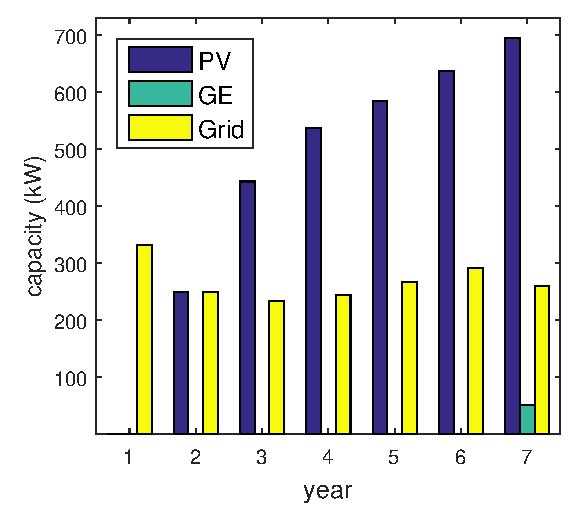
\includegraphics[width=0.32\columnwidth]{figs/long_term_capacity}}
 \label{f.capacity_annual_change}}
 \subfigure[Expenditures]{{\includegraphics[width=0.32\columnwidth]{figs/long_term_cost}}
 \label{f.cost_annual_change}}
 \subfigure[Normalized emissions]{{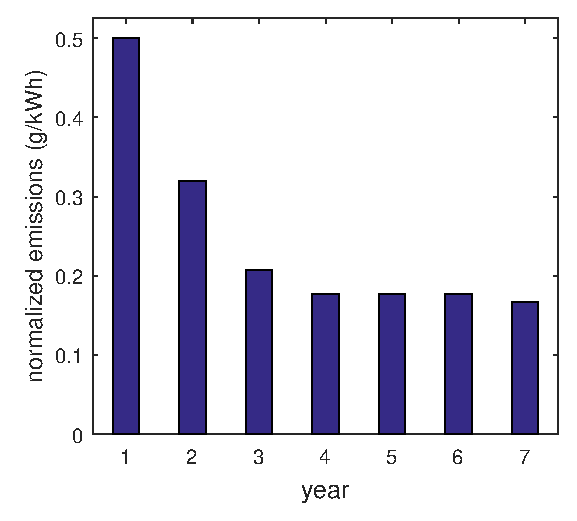
\includegraphics[width=0.32\columnwidth]{figs/long_term_co2_norm}}
 \label{f.co2_annual_change}} 

 \caption{Annual capacity planning. The data center is going to use more PV generation and GE generation while reducing the imported energy from the electricity grid. The major expenditure concentrates on the infrastructure of PV. The normalized emissions go down due to the high penetration of PV generation.}
 \label{f.annual_change}
 \end{center}

\end{figure*}
}
In this subsection, we evaluate the joint framework on planning and operating a sustainable data center. We answer three questions: How does the optimization framework plan annually? How much benefits can the optimization framework achieve? How do prediction errors impact on the proposed framework?

\textbf{Annual capacity planning.} In practice, the electricity prices, gas prices, and workload demand tend to increase in the long-term. The average annual-increasing rates of electricity prices, gas prices, and workload demand are $1.05$, $1.01$, and $1.09$ \cite{eiaElectricityPrices,gasPrice,StevenGlobalTraffic}. Meanwhile, the amortized cost of PV array decreases 12\% annually \cite{solarCost}.

Figure~\ref{f.capacity_annual_change} presents the capacities of power sources in 7 years. In general, the data center increases the capacity of PV annually but not the peak grid power consumption. In the first year, the data center prefers the electricity grid to other power sources because of the low electricity price. However, the data center significantly expands PV generation capacity from year 2 as the electricity prices increase and the infrastructure cost of PV decreases. In year 7, the data center provisions GE generation since the slow natural gas becomes relatively cheaper than the imported electricity. Although the data center prefers to use PV, the peak grid power consumption is still noticeably large. The intuition behind this is that PV generation is not available during night time which requires the data center to provision grid power.

Figure~\ref{f.cost_annual_change} shows the annual breakdown expenditures of the data center. In the first year, the utility bill (Util) of the imported energy from the electricity grid is dominant. Meanwhile, the cost of PV infrastructure (PV-I) quickly increases because PV amortized cost is added by installing more PV every year. The PV O\&M (PV-O) expenditure linearly increases as the PV capacity goes up. In year 7, the GE O\&M cost (GE-O) is 15\% the total annual expenditure. GE-O mainly comes from the amount of natural gas supplied to the GE.

The annually normalized emissions of the data center, defined as the ratios of total emissions to the total power demand, are plotted in Figure~\ref{f.co2_annual_change}. Since the normalized emissions of the electricity grid are high, the normalized emissions of the data center are highest in year 1.
The increase of the PV generation can reduce normalized emissions for the data center. The normalized emissions sharply go down to 36\% in year 4 as compared to the first year. However, there is little change from year 4 to year 7 as the ratio of PV capacity to other power sources is not considerably decreased.

\hideit{
\begin{figure*}[!ht]
 \begin{center}
	 \subfigure[Grid-only (GRID)]{{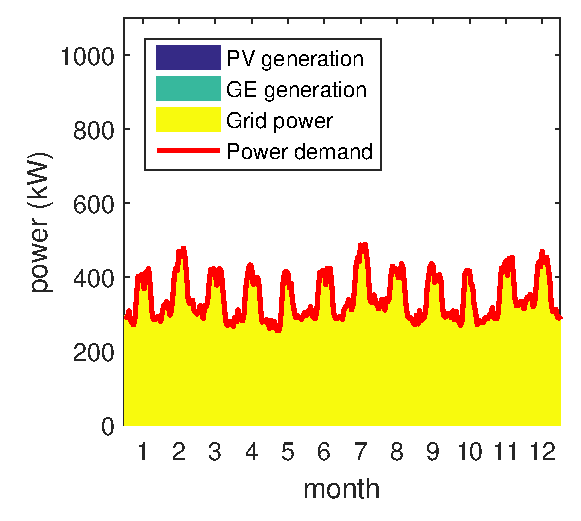
\includegraphics[width=0.32\columnwidth]{figs/nz-grid_year}}
	 \label{f.grid}}
	 \subfigure[Supply-only (SUP)]{{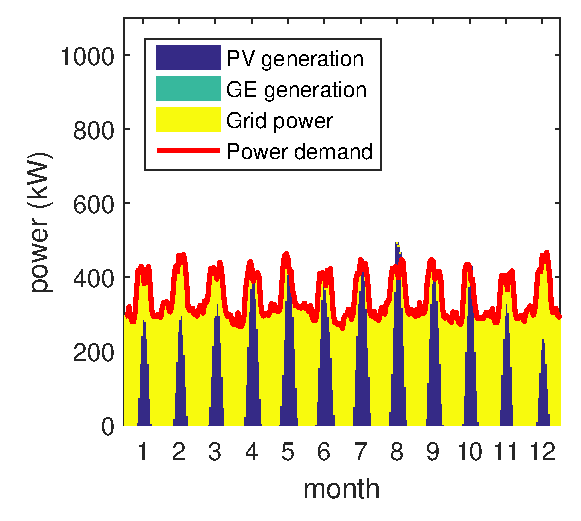
\includegraphics[width=0.32\columnwidth]{figs/nz-supply_year}}
	 \label{f.supply}}
	
	 \subfigure[Demand-only (DEM)]{{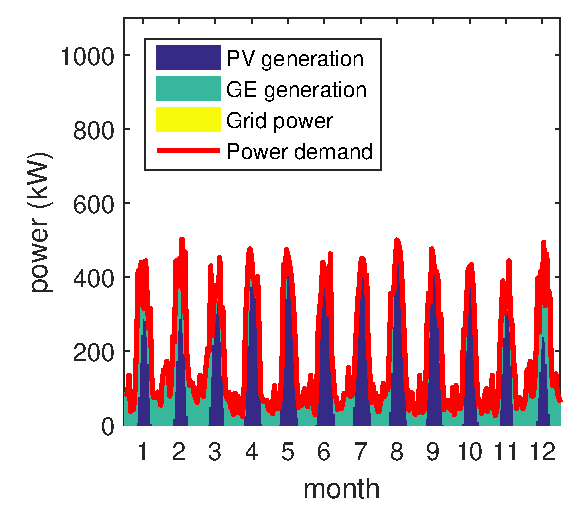
\includegraphics[width=0.32\columnwidth]{figs/nz-demand_year}}
	 \label{f.demand}}
	 \subfigure[Proposed (PROP)]{{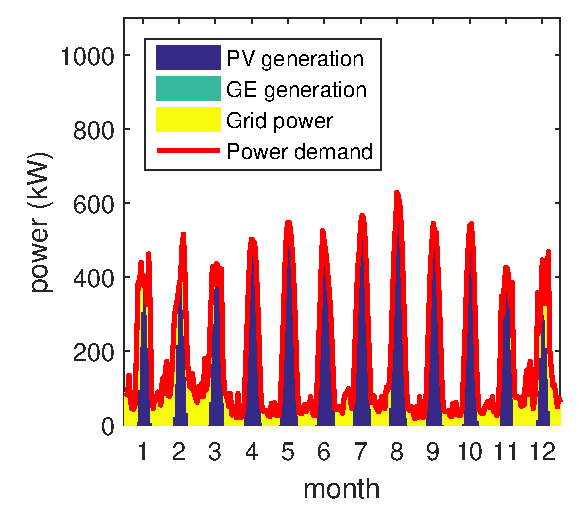
\includegraphics[width=0.32\columnwidth]{figs/nz-int_year}}
	 \label{f.integrated}}

 \caption{The power profiles of the baseline methods and the proposed framework in year 5. GRID provisions the only grid power. SUP optimizes the power sources only at the supply side. DEM optimizes the power demand, i.e., scheduling the batch jobs. } 
 \label{f.behaviors}
 \end{center} 

\end{figure*}
}

\textbf{How much cost savings and emission reductions does the proposed framework achieve?} To highlight the benefits of the proposed framework, we compare the proposed framework (PROP) with three baseline methods, namely grid-only, supply-only, and demand-only. 
\begin{itemize}

 \item Grid-only (GRID): \new{The grid-only method only uses the grid power from the electricity grid to provision the power demand. It does not use any power demand management techniques.}

 \item Supply-only (SUP): Given the power demand, the supply-only method optimizes capacity planning at the supply side.
This method can optimize the use of energy sources among PV, GE, and the public electricity grid. 

 \item Demand-only (DEM): \new{At the supply side, the capacities of PV and GE generation are set at 50\% and 70\% of the power demand capacity, respectively. 
The demand-only method optimizes the power demand, i.e., scheduling the batch jobs, to reduce the operational cost.}

\end{itemize}
In fact, PROP combines the SUP and DEM, and therefore can provide the best cost reductions.

The power profiles of these four methods in twelve typical days representing for the twelve months in year 5 are shown in Figure \ref{f.behaviors}.
GRID provisions power only from the electricity grid. SUP prefers the PV sources to the electricity grid and GE. Meanwhile, DEM utilizes installed GE generators because the electricity price is relatively more expensive than the O\&M cost of GE sources. However, PROP uses only PV generation and grid power. In Figure \ref{f.demand} and \ref{f.integrated}, DEM and PROP shape the power demand to follow the PV generation while GRID and SUP are dependent on imported electricity.
\hideit{
\begin{figure}[!th]
 \begin{center} 
 % \subfigure[Capacities]{{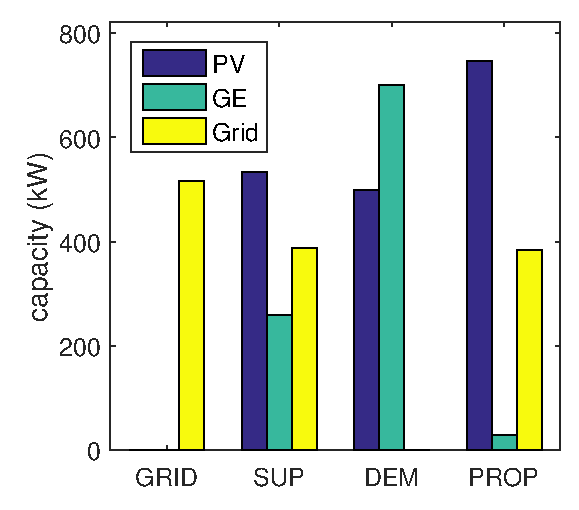
\includegraphics[width=0.48\columnwidth]{figs/capacity_comparison}}
 % \label{f.capacity_comp}}
 % \hspace{0.5cm}
 \subfigure[Expenditures]{{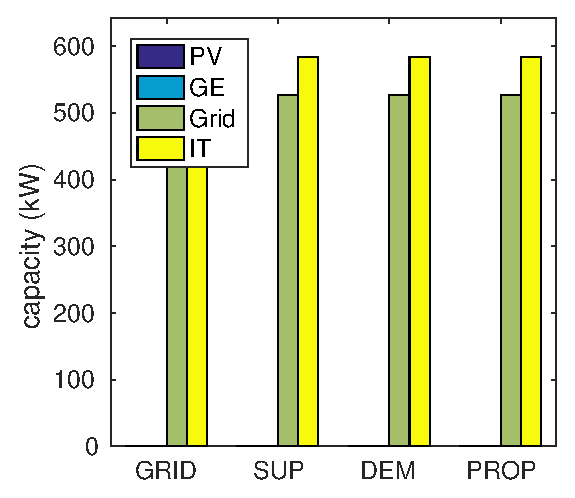
\includegraphics[width=0.32\columnwidth]{figs/cost_comparison}}
 \label{f.cost_comp}}
 % \hspace{0.5cm}
 \subfigure[Emissions]{{\includegraphics[width=0.32\columnwidth]{figs/emission_comparison}}
 \label{f.co2_comp}} 

 \caption{Comparisons with baseline methods. The proposed framework reduces up to 50\% of the total expenditures, and significantly cuts down 75\% greenhouse gas emissions.} 
 \label{f.basic}

 \end{center}
\end{figure}
}

We evaluate the four methods in terms of costs and emissions in Figure \ref{f.basic}. It shows that PROP remarkably reduces the total expenditure by 50\% while it achieves very close emissions to the lowest one, i.e., DEM. In Figure \ref{f.cost_comp}, SUP slightly reduces the total cost as it still depends much on the electricity grid. However, DEM shows that power management at demand side is very effective because it makes the power demand follow the PV generation.

\delete{\textbf{Should we provision IT capacity?} In order to highlight the importance of optimizing IT capacity, we carry out an experiment that plans the capacities of IT capacity and power sources. In Figure {\ref{f.IT}}, the IT capacities in the four methods are different. The proposed framework allows data center operators to provision the smallest IT capacity compared to other baseline methods. Consequently, the proposed framework can significantly reduce the total expenditure. Hence, the capacity of IT plays an important role reducing the total cost of ownership.}

\del{
	\begin{figure}[!htbp]
		\begin{center}
			\subfigure[Capacity]{{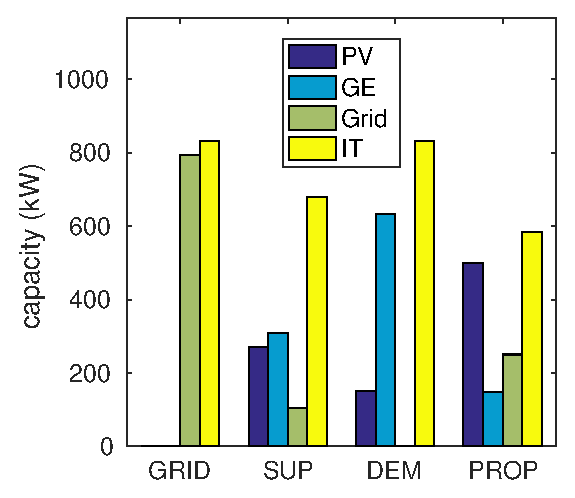
\includegraphics[width=0.48\columnwidth]{figs/capacity_IT}}
				\label{f.capacity_IT}}
			\subfigure[Cost]{{\includegraphics[width=0.48\columnwidth]{figs/cost_IT}}
				\label{f.cost_IT}}
			\caption{Comparisons with different baselines when IT capacity is also optimized. The IT capacitiy plays an important role in capacity planning.}
			\label{f.IT}
		\end{center}
	\end{figure}}


\textbf{\textit{Key insights}}: (i) The proposed framework not only remarkably reduce the total cost, but also utilizes renewable energy very well. (ii) As the renewable installation becomes more cost-effective, the proposed framework prefers to use renewable energy and reduce the dependence of sustainable data centers on the electricity grid. 
%\delete{(v) If we have opportunity to optimize IT subsystem, this can have considerate impact on the total annual expenditure of the data center.}

\subsection{Impacts of prediction errors}
\label{sec:ImpactOfPredictionErrors}

%Since the capacity planning of a data center is executed in the long-run, it suffers from prediction errors.

%To study the impact prediction errors on capacity planning
Prediction errors are generally negligible during operational management, which happens in real-time. Hence, GRID and DEM are not affected by the prediction errors because they do not need capacity planning. On the other hand, SUP and PROP suffer from prediction errors because they provide the capacity planning decisions, and then operate the data center in real-time based on the planned capacities. We normalize the root mean squared errors (RMSE) compared to the means of interactive workloads, batch jobs, capacity factors of PV, electricity prices, and gas prices, respectively. For instance, when normalized RMSEs are $0.2$, the RMSEs of all the aforementioned predictions are 20\% of their means. 

Figure {\ref{f.cost_err_comparison}} shows the impacts of prediction errors on the total expenditures of the four methods. As the prediction errors become large (more than 10\%), the total costs of SUP and PRO go up while the costs of GRID and DEM stay unchanged. Interestingly, total cost of the proposed framework is still the best and achieves the significant cost savings, i.e., 58\% of GRID. The intuition behind this is that the operational management is cost-efficient in using the various power sources and scheduling the batch jobs to compensate for the prediction errors.

The impacts of prediction errors on emissions are presented in Figure {\ref{f.emission_err_comparison}}. As the prediction errors increase, the emissions of PROP go up. However, PROP still reduces 49\% of emissions reduction compared to GRID. Specially, the emissions stay unchanged when RMSE is greater than 0.2.
%The curve of the supply-only method is more interesting. It first does not change much at normalized errors less than $0.05$, goes up from $0.05$ to $0.25$, and finally goes down as the normalized errors greater than $0.25$. Because of prediction errors, the supply-only method over-provisions the PV capacity. When the prediction errors are too small, the over-provisioned PV capacity is useful in reducing the emissions. When the normalized errors become larger, the supply-only method uses more electricity grid to compensate the renewable energy which causes more emissions. However, when the electricity prices are very unpredictable, it prefers the gas engines that release less emissions than the public electricity grid.

\hideit{
\begin{figure}[!th]
	\vspace{-0.1cm}
 \begin{center} 
 \subfigure[Expenditures]{{\includegraphics[width=0.32\columnwidth]{figs/cost_err_comparison}}
 \label{f.cost_err_comparison}} 
 \subfigure[Emissions]{{\includegraphics[width=0.32\columnwidth]{figs/emission_err_comparison}}
 \label{f.emission_err_comparison}} 
 \caption{Impacts of prediction errors. Under large prediction errors, the proposed framework still achieves the significant cost and emission reductions.} 
 \label{f.prediction}
 \end{center}
  \vspace{-0.3cm}
\end{figure}
}
\textbf{\textit{Key insights}}: Under large prediction errors, our proposed framework still achieves significant cost and emission reductions compared to the baseline methods.

\subsection{Sensitivity analysis}
\label{sec:netzero_evaluation}

We carry out the experiments based on a real data center, called Net-zero Energy Data Centers (NEDC) invented by HP \cite{arlitt2012towards}. 
In NEDC, the total local generation (i.e. PV and GE generations) is greater than the total power consumption. NEDC have an additional constraint
$$\sum_{t=1}^{T}\sum_{r=1}^{R}c_{r}(y,t) + \sum_{t=1}^{T}\sum_{s=1}^{S}c_{s}(y,t) \geq \sum_{t=1}^{T}P(y,t), \quad \forall y,$$
where the left hand side and the right hand side are the total power generation and the total power consumption in year $y$, respectively.

We focus on studying the impacts of supply and demand factors on the data centers during the first year. The supply factors include electricity price, and gas price. The demand factors include shape of interactive workload and ratio of flexible workload. Besides the capacities and expenditures of the data center, we study the payback period, which is the number of years for the data center to recoup the investment in the infrastructure costs of PV and GE instead of using only the electricity grid. The shorter payback period is, the more financial benefit the proposed framework provides.

\subsubsection{Impacts of supply factors}

\hideit{
\begin{figure}[!ht]
%matlab: TCO_grid_electricity_0115.m
\vspace{-0.1cm}
\begin{center}
	\subfigure[Capacity]{{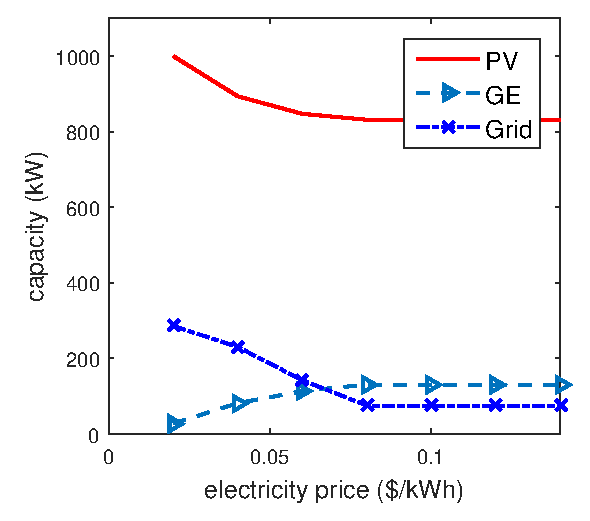
\includegraphics[width=0.32\columnwidth]{figs/capacity_electricity}}
		\label{f.capacity_electricity}}
	\subfigure[Payback period]{{\includegraphics[width=0.32\columnwidth]{figs/payback_electricity}}
		\label{f.payback_electricity}}
	\caption{Impacts of electricity prices. As the electricity price increases, the capacity of GE is increased to compensate for the PV generation during nighttime. Interestingly, it results in reducing the capacity of PV.}
	\label{f.electricity}
\end{center}
\vspace{-0.3cm}
\end{figure}
}

\emph{Electricity price}. Figure~\ref{f.electricity} presents the impacts of electricity prices on the proposed framework. Figure~\ref{f.capacity_electricity} shows that the data center uses more GE generation and less grid power when the electricity price increases. However, the data center surprisingly keeps reducing the capacity of PV. It is because the data center starts to use more GE to provide power during nighttime and replace PV during daytime. It is because the costs of GE are relatively lower than the infrastructure of PV as PV is not fully utilized around its peak generation. In addition, when the grid power becomes more expensive, the payback period sharply decreases as in Figure \ref{f.payback_electricity}. Hence, the NEDC can significantly gain financial benefits when the electricity prices are high.
\hideit{
\begin{figure}[!ht]
%	\vspace{-0.3cm}
\begin{center}
	\subfigure[Capacity]{{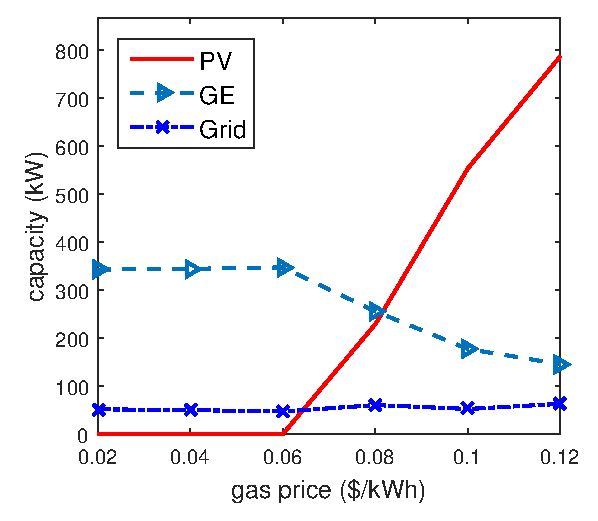
\includegraphics[width=0.32\columnwidth]{figs/capacity_gas}}
		\label{f.capacity_gas}}
	%        \subfigure[Cost]{{\includegraphics[width=0.48\columnwidth]{figs/cost_gas}}
	%            \label{f.cost_gas}}
	\subfigure[Payback period]{{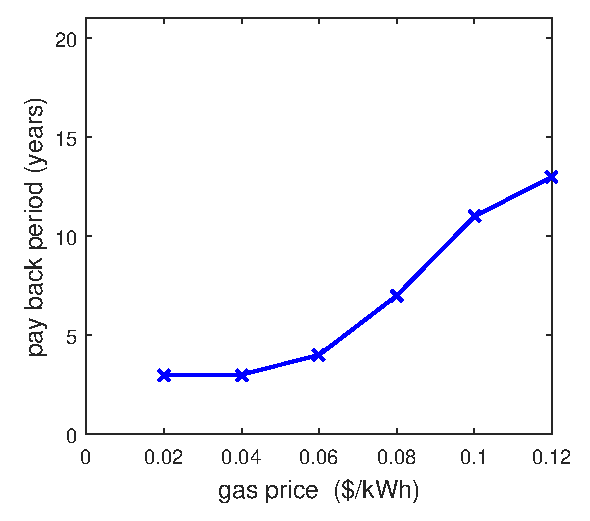
\includegraphics[width=0.32\columnwidth]{figs/payback_gas}}
		\label{f.payback_gas}}
 \vspace{-0.3cm}
	\caption{Impacts of gas prices. As the gas prices increase, the capacity of PV increases quickly because the data center cannot import too much electricity grid.}
	\label{f.gas}
\end{center}
\vspace{-0.3cm}
\end{figure}
}
\emph{Gas price.} Figure~\ref{f.gas} shows the impacts of gas prices on capacities and payback periods. In Figure \ref{f.capacity_gas}, the data center should use the GE generation at low gas prices, but it switches using PV when the gas price is more expensive. Especially, there is the sharp increase of PV capacity when the gas price is greater than $0.06$. Due to the non-dispatchability of solar energy, the data center needs the large capacity of PV generation to compensate for the reduction of GE generation. As the gas price increases, the payback period goes up as in Figure \ref{f.payback_gas} because the data center needs more PV.

\begin{figure}[!ht]
	%matlab: TCO_grid_payback_pv.m or TCO_grid_surface.m
	\begin{center}
		\subfigure[Capacity]{{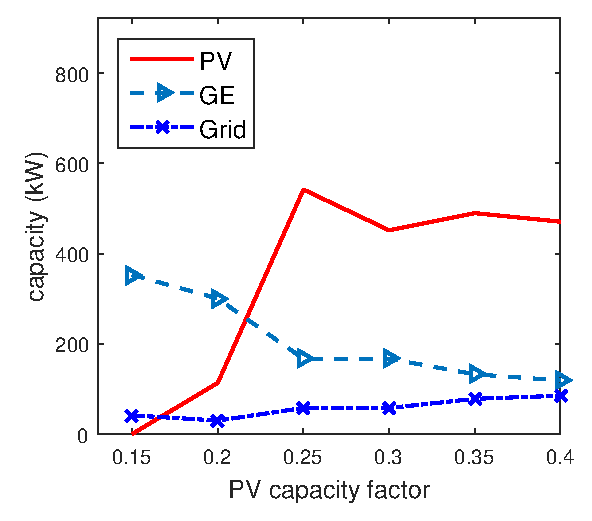
\includegraphics[width=0.32\columnwidth]{figs/capacity_PV}}
			\label{f.capacity_PV}}
		%        \subfigure[Cost]{{\includegraphics[width=0.48\columnwidth]{figs/cost_PV}}
		%            \label{f.cost_PV}}
		\subfigure[Payback period]{{\includegraphics[width=0.32\columnwidth]{figs/payback_PV}}
			\label{f.payback_PV}}
		\caption{Impact of different PV capacity factors. The curves of PV are very interesting which goes up and down because the high capacity factors have strong impact on the capital cost and operational cost of PV.}
		\label{f.PV}
	\end{center}
\end{figure}

\new{
	\emph{PV capacity factor.} To understand how PV capacity factors affect on the proposed framework, we run the experiments with various capacity factors of PV.
	Recall the capacity factor is the average power generated, divided by the rated peak power. Figure {\ref{f.PV}} shows the dependence of the capacities and payback periods of the data center on PV capacity factors. The capacity of PV increases and then varies at high capacity factors. The capacity factor of PV array varies due to diverse reasons, such as geographical conditions. When PV has enough efficiency, i.e. capacity factor varies from 0.15 to 0.25, the data center starts to use PV. At a very high capacity factor (0.25-0.4), it is not necessary to increase the PV capacity because even the lower capacity with high capacity factors can still provide enough generation.}

\textbf{\textit{Key insight}}: The capacities of PV, GE, and peak power of grid power consumption adapt to the variety of supply factors accordingly. (i) The impacts of electricity prices and gas prices show the trade-offs between PV and GE. (ii) Under the increase of electricity price, the capacity of PV unexpectedly goes down together with the peak grid power.	(iii) Under a certain gas price, the data center does not provision PV generation but only use GE and grid power instead.\delete{(iii) The impacts of PV capacity factors are complicated. Even at very high capacity factors, other power sources like GE and electricity grid play a crucial role to additionally supply the data center because PV is not available during nighttime.}

%%%%%%%%%%%%%%%%%%%%%%%%%%%%%%%%%%%%%%%%%%%%%%%%%%%%%%%%%%%%%%%%%%%%%%%%%%%%%%%%%%%%%%%%

\subsubsection{Impacts of demand factors.}

Besides the supply factors, it must be interesting to study how the demand factors impact on capacity planning and costs of the data center.
\hideit{
\begin{figure}[!ht]
	\vspace{-0.3cm}
	%matlab: TCO_grid_payback_PMR.m
	\begin{center}
		\subfigure[Capacity]{{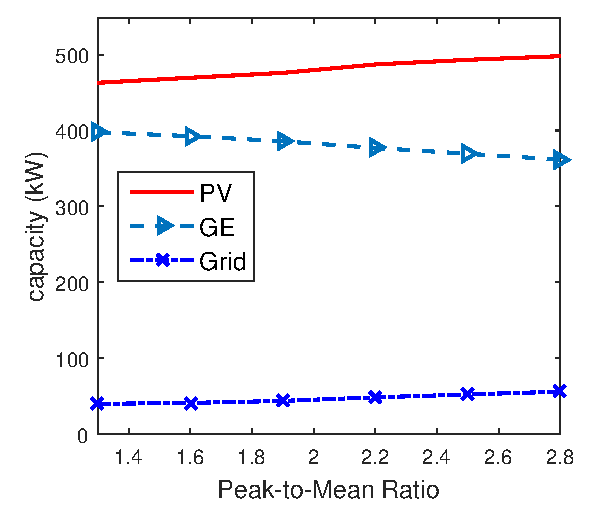
\includegraphics[width=0.32\columnwidth]{figs/capacity_PMR}}
			\label{f.capacity_PMR}}
		\subfigure[Cost]{{\includegraphics[width=0.32\columnwidth]{figs/cost_PMR}}
			\label{f.cost_PMR}}
		%\subfigure[Payback period]{{\includegraphics[width=0.48\columnwidth]{figs/payback_PMR}}
		\caption{Impacts of interactive workload shapes. The shapes of interactive workload have limited impacts on the capacities and expenditures of GE and PV.}
		\label{f.PMR}
	\end{center}
 \vspace{-0.3cm}
\end{figure}
}

\emph{Shape of interactive workload:} Interactive workload is non-flexible and required to be processed with high responsive speed in data centers. We use the peak-to-mean ratio (PMR) to study the impacts of interactive workload shape. Figure \ref{f.PMR} shows that shape of interactive workload has limited influence on both the capacities and expenditures of data centers. In particular, the capacity of PV and the peak grid power consumption slightly increase as the PMR increases. On the other hand, the data center slightly reduces GE when it has more PV power generation. As the capacities of PV and GE do not vary much, the breakdown expenditures are almost the same when varying the PMRs in Figure {\ref{f.cost_PMR}}.

\hideit{
\begin{figure}[!ht]
%matlab: TCO_grid_payback_ratio.m
\begin{center}
	\subfigure[Capacity]{{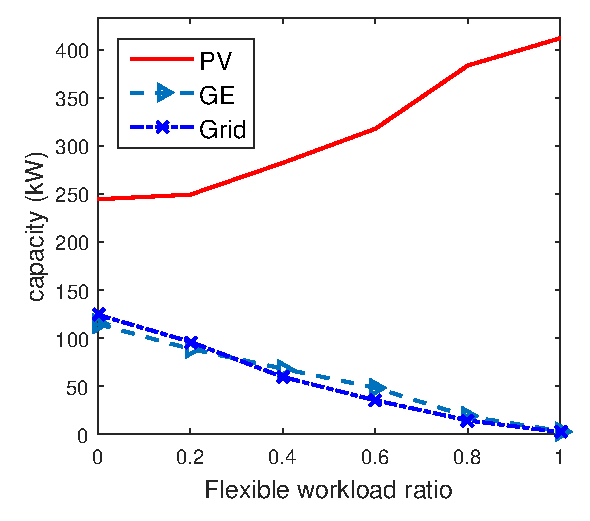
\includegraphics[width=0.32\columnwidth]{figs/capacity_batch}}
		\label{f.capacity_batch}}
	\subfigure[Cost]{{\includegraphics[width=0.32\columnwidth]{figs/cost_batch}}
		\label{f.cost_batch}}
	%\subfigure[Payback period]{{\includegraphics[width=0.48\columnwidth]{figs/payback_batch}}
	%\label{f.payback_batch}}
	\caption{Impacts of flexible workload ratios. The ratio can significantly reduces the total expenditure and change the capacity structure of the data center.}
	\label{f.batch_ratio}
\end{center}
\end{figure}
}
\emph{Ratio of flexible workload} is the ratio of batch jobs to the IT workload demand. The higher ratio of flexible workload means the more flexibility data centers have in power demand management. In particular, Figure~\ref{f.capacity_batch} highlight that the data center is more aggressive in using renewable energy as the ratio of flexible workload increases. It shows that the flexible workloads can promote the use of renewable sources. Especially, when workloads are totally flexible, there is no need to use GE and grid power as the workloads can be scheduled to totally follow PV generation. Figure~\ref{f.cost_batch} shows that the flexible workloads can significantly reduce the total expenditure, e.g., 28\% reduction of the total cost.

\textbf{\textit{Key insights}}: (i) The shape of interactive workload does not affect much on the capacity planning and operational management of data centers. (ii) The flexible workloads promote the use of renewable energy and significantly reduces the total cost.

\section{Data center demand response}
\label{sec:DR_evaluation}

In this section, we extend the framework to study data center demand response (DCDR).


\subsection{Modeling data center demand response}
\begin{table}[!ht]
	\tbl{Demand response rates.\label{tbl:DR_rates}}{
	\begin{tabular}{|c|c|}
		\hline
		\textbf{Symbol}  &  \textbf{Value} (\$/kWh) \\ \hline \hline    
		
		$p_{tou}(t)$  & 0.05 (night), 0.219 (peak), 0.06 (off) \\     \hline
		$p^l_{ibr}$   & 0.2 ($l=1$: 50kW), 0.5 ($l=2$: 100kW), \\  \hline        
		$p_{cpp}$     & 11.2 \\ \hline
		$p_{sr}$      & 0.02  \\ \hline
		$p_{ws}$      & 0.05 \\ 
		\hline
	\end{tabular}}
\end{table}

To model DCDR, the proposed framework is modified for including the costs of participating in DR programs into the objective function a part of \textit{UtilBill}. In particular, we consider the following five DR programs:
\begin{itemize}
	\item Time-of-Use (ToU) rates, $p_{tou}(t)$, are defined based on the different times during a day, such as night time, peak time, and off-peak time \cite{ToURates}.
	\item Inclining block rates (IBR) encourage customers to consume electricity under some level, $l$, by charging a higher price, denoted by $p^l_{ibr}$, for the exceeding electricity usage.
	\item Under coincidence peak pricing (CPP) programs, industrial consumers like data centers are charged at a very high price, $p_{cpp}$, (e.g. than 200 times) for the usage during coincident peaks \cite{liu2013data}. For example, the CPP time is an hour per month selected by the utility company.
	\item In spinning reserve (SR) service, electricity customers are rewarded based on predefined SR rates if they reduce their load after receiving an SR signal command. 
	\item The rates $p_{ws}$ in wholesale markets are typically cheaper than the regular electricity prices. The participations of data centers in wholesale markets allow electricity suppliers to efficiently plan their generation.
\end{itemize}
The DR rates are summarized in Table \ref{tbl:DR_rates}.

\subsection{Numerical results}
\hideit{
\begin{figure*}[!ht]
	\begin{center} 
		\subfigure[Without DR programs. Data centers only use the grid power as the base prices of electricity are cheap. ]{{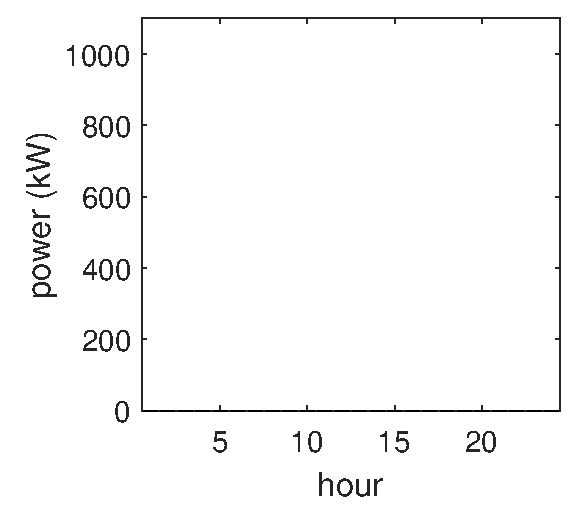
\includegraphics[width=0.32  \columnwidth]{figs/nz-int_NoDR}} 
			\label{fig:No_DR_program}    }
		\subfigure[Time of Use (ToU). Data centers provision 3 types of power sources during peak-hours.]{{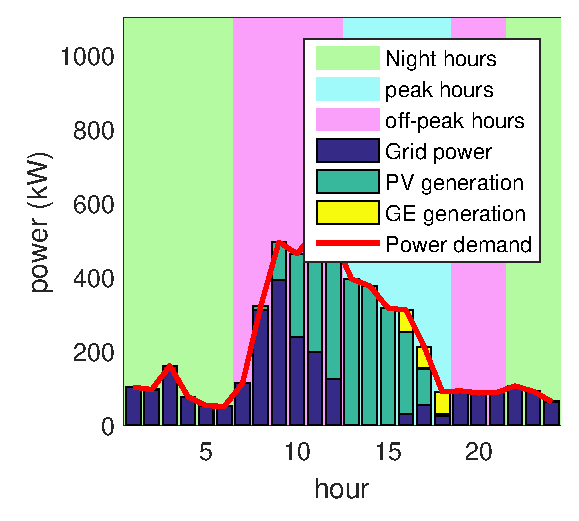
\includegraphics[width=0.32  \columnwidth]{figs/nz-int_tou}} 
			\label{fig:DR_programs_tou}   }
		\subfigure[CPP. Data centers prefer to use GE generation and PV generation in CPP hours.]{{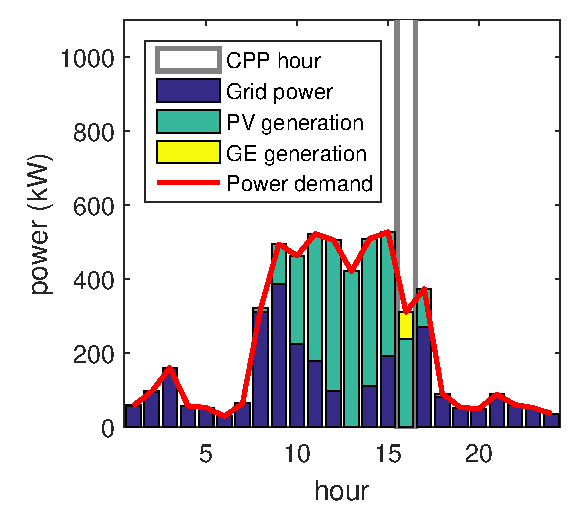
\includegraphics[width=0.32 \columnwidth]{figs/nz-int_cpp}} 
			\label{fig:DR_programs_cpp}    }
		\subfigure[IBR. The data center almost provisions its grid power under the IBR levels. ]{{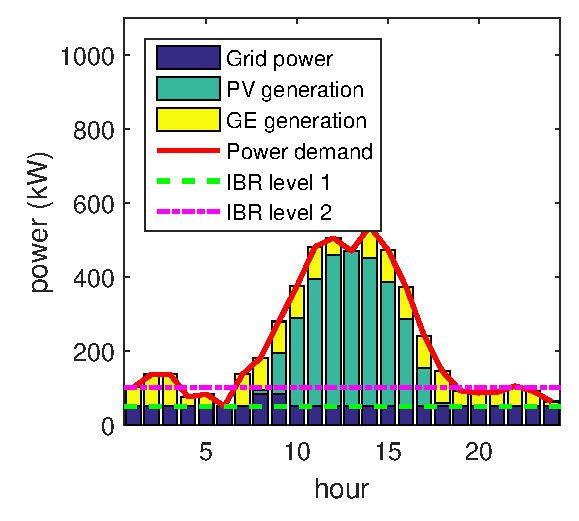
\includegraphics[width=0.32  \columnwidth]{figs/nz-int_ibr}} 
			\label{fig:DR_programs_ibr}    }
		\subfigure[Spinning reserve (SR). The data center reduces the grid power during SR hour to earn the SR reward. ]{{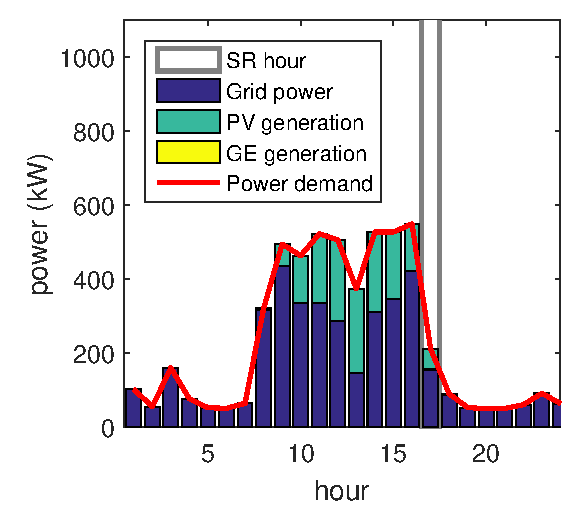
\includegraphics[width=0.32  \columnwidth]{figs/nz-int_sr}} 
			\label{fig:DR_programs_sr}    } 
		\subfigure[Wholesale (WS). The data center flattens the power demand to follow the pre-purchased power.]{{\includegraphics[width=0.32  \columnwidth]{figs/nz-int_BiMarkets}} 
			\label{fig:DR_programs_BiMarkets}    }        
		\caption{The power profiles of the data centers participating in different DR programs.}         
		\label{fig:DR_power_profiles}
	\end{center}
\end{figure*}

\begin{figure*}[!h]
	\begin{center}
		\subfigure[Capacity]{{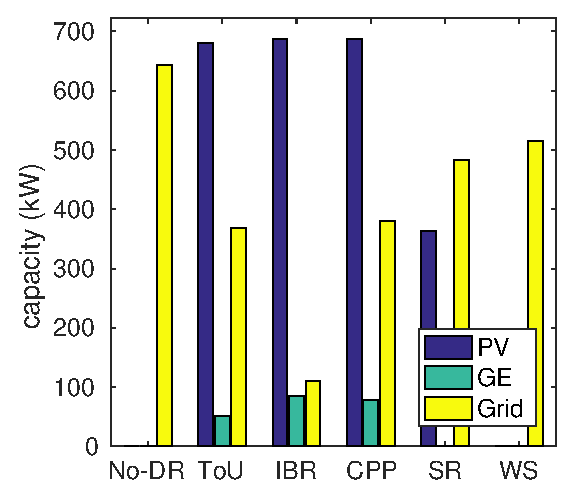
\includegraphics[width=0.32  \columnwidth]{figs/capacity_int_DR}} 
			\label{fig:DR_programs_capacity}    }
		\subfigure[Expenditures]{{\includegraphics[width=0.32  \columnwidth]{figs/cost_int_DR}} 
			\label{fig:DR_programs_cost}    }
		\subfigure[Emissions]{{\includegraphics[width=0.32  \columnwidth]{figs/emission_int_DR}} 
			\label{fig:DR_programs_emission}    }
		\caption{Impacts of DR programs on capacities, expenditures, and emissions of the data center. }         
		\label{fig:DR_programs}
	\end{center}
	\vspace{-0.5cm}
\end{figure*}
}
The numerical results are to study the impacts of DR programs on a data center using our proposed framework within a year. We answer the following two questions: How does the power profile of data center look like when participating in DR programs? How do DR programs impact on costs and emissions? 

Figure \ref{fig:DR_power_profiles} presents the typical daily power profiles of data centers participating in the DR programs. There are six cases: (1) Data centers do not participate in any DR programs, and data centers participate in (2) the ToU pricing program, (3) the CPP program, (4) the IBR program, (5) the SR ancillary service program, and (6) the wholesale market.

In the case of without any DR programs in Figure \ref{fig:No_DR_program}, the data center prefers to provision only the grid power because the electricity price is relatively cheaper than using GE and PV. In addition, the proposed framework does not need to schedule the batch jobs as the electricity price is fixed.

Figure \ref{fig:DR_programs_tou} illustrates the power profiles of the data center in the ToU program. We have 3 ToU price levels for off-peak hours $\$0.06/kWh$, night hours $\$0.05/kWh$, and peak hours $\$0.219/kWh$ \cite{Shahan2011ToUTexas}. The rates of night hours are the cheapest while the electricity rates of peak hours are the most expensive. The data center provisions PV and GE generation to reduce the electricity bill during peak hours. As the peak of PV generation is in the peak hours, PV generation contributes the most power during peak hours. Compared to Figure \ref{fig:No_DR_program}, the power demand is shifted to match the PV generation and avoid the high peaks during the peak hours. When the PV generation goes down within the ToU peak hours, the data center operates GE to serve the power demand. During off-peak hours, the data center prefers to use PV generation if available, then imports the energy from the electricity grid if necessary. Furthermore, the peak of power demand is not at the peak hours compared to the case of without any DR programs. However, why does the data center not shift the power demand from the off-peak hours (7 am - 12 pm) to the night hours (9 pm 6 am)? Because the interactive workload and batch jobs are colocated in the same servers, scheduling the batch jobs may increase the idle power.

Figure \ref{fig:DR_programs_cpp} shows the case of the data center participating in the CPP program. During the CPP hour, the data center needs to avoid using the grid power because the CPP rate is too high. Therefore, the data center provisions GE generation and utilizes PV generation during the CPP hour. A larger amount of PV generation is used compared to the case without DR programs. The power demand management schedules the batch job workload to react to the shape of PV generation, which has the peak in the afternoon.

We study the power profile of the data center with respect to two IBR levels which are level 1 (50kW) and level 2 (100kW) as in Figure \ref{fig:DR_programs_ibr}. The electricity prices of exceeding the level 2 grid power is $\$0.5$/kWh, more expensive than the level 1, i.e., $\$0.2$/kWh.  The idea of IBR is to regulate the power demand under the two load levels. As we expected, the data center adapts to the IBR program very well. In particular, the grid power is mostly under the level 1 and never exceeds the level 2. In order to provision power under the IBR levels, the data center actually requires a lot of PV generation and GE generation. The batch job workload is shifted to the high peak of PV generation during day time. On the other hand, GE is used in the whole day.

Figure \ref{fig:DR_programs_sr} presents the operation of the data center in the SR program. In the SR program, the data center can earn financial benefits if it reduces the power demand compared to the baseline consumption. In this simulation, the baseline consumption is the power consumption of the data center without participating in any DR program. We run the optimization framework to minimize the total cost for the data center in the DR program. During the SR hour, the data center reduces 30\% their grid power consumption as compared to the case without DR programs.

In the wholesale market, it is assumed that the data center provisions 200kWh every hour at a cheaper price (0.05 \$/kWh) than the base price (0.056 \$/kWh). The power profile of data center is in Figure \ref{fig:DR_programs_BiMarkets}. It is seen that the power demand is flattened to follow the pre-purchased electricity in the wholesale market. The data center significantly reduces its peak compared to the case without DR programs, which can be very beneficial to reduce the peak demand of the electricity grid.

The comparison of the six cases of data center demand response in terms of capacities, costs, and emissions are shown in Figures \ref{fig:DR_programs}. In general, the proposed framework enables the data center to adapt to each DR program very well. The data center increases the capacities of GE and/or PV under the ToU, CPP, IBR, and SR programs as in Figure \ref{fig:DR_programs_capacity}. Hence, the DR programs can indirectly change the capacity planning of data centers.
In Figure \ref{fig:DR_programs_cost}, the total costs of the data center increase in the ToU, IBR, and CPP programs but they decrease in the SR program and the wholesale market. The lowest expenditure is in the wholesale market because of the cheap electricity price but it releases the most emissions as the grid power is generated by mainly using the fossil fuel. Participating in ToU, IBR, and CPP programs causes the data center spends slightly more expenditures, but data centers can remarkably reduce emissions by using other environmentally friendly power sources rather than the grid power. 

\textbf{Key insights:} The proposed framework enables data centers to adapt to DR programs very well. (i) The data center uses a lot of PV and/or GE generation under ToU, IBR, CPP, and SR. (ii) While the total cost of the data center slightly increases in the ToU, CPP, and IBR programs, it can be reduced in the SR program and wholesale market. (iii) Data centers participating in ToU, IBR, CPP, and SR programs can cut down their emissions by provisioning other power sources rather than grid power.

\section{Conclusions and future work}

In this paper, we propose an optimization framework for joint capacity planning and operational management that not only plans the capacities for sustainable data centers but also takes the operational management into account. The proposed framework can actually cut down significant expenditures by integrating the optimizations on both supply and demand sides. 
Numerical evaluation based on real-world case studies highlights the benefits to data center operators by using the proposed framework. In particular, it can achieve up to 50\% cost savings and 75\% emission reductions. 

There are a lot of interesting future directions. For instance, tackling the stochastic characteristics of workload and renewable energy in capacity planning and operational management is challenging and important. Another promising direction is to extend the framework from a single data center to the system of geographically distributed data centers, which has more flexibility on planning their IT capacities because the workload demand can be shifted among different data centers. These can result in further cost and emission reductions.

\section*{Acknowledgments}

Part of this work  was done when Zhenhua Liu visited Hewlett Packard Labs. This work is partially supported by NSF through CNS-1464388 and the MSIP ``ICT Consilience Creative Program" (IITP-2015-R0346-15-1007) of Korea.



% Bibliography
\bibliographystyle{ACM-Reference-Format-Journals}
\bibliography{bib/DCDR}

% History dates
\received{February 2007}{March 2009}{June 2009}

% Electronic Appendix
%\elecappendix

\medskip


\end{document}
% End of v2-acmsmall-sample.tex (March 2012) - Gerry Murray, ACM


